%-------------------------------------------%
\newpage
\section{PID Control}
%-------------------------------------------%

%-------------------------------------------%
\subsection{Open-loop Control} 
%-------------------------------------------%
\begin{itemize}
    \item No feedback in open-loop control, output has no effect on the control action;
    
    \item Open-loop control is convenient when it is hard to measure output;
    
    \item It is only used if the uncontrolled plant dynamics is \textbf{perfectly known} and is not subject to any environmental changes.
\end{itemize}

\begin{figure}[H] 
    \centering 
    % 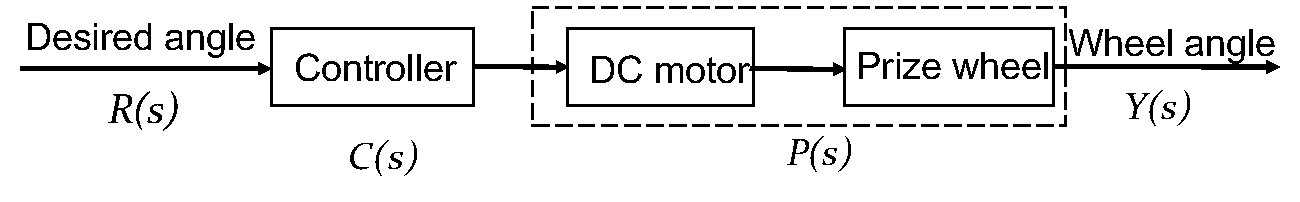
\includegraphics[width=.7\textwidth]{images/open-loop.pdf}
    \begin{tikzpicture}[auto, node distance=2cm,>=latex',line width=1pt]
    \node [input, name=input] {};
    \node [block, right of=input] (controller1) {controller};
    \node [block, right= 1cm of controller1] (controller2) {DC motor};
    \node [block, right= 1cm of controller2] (controller3) {prize wheel};
    \node [output, right=1.5cm of controller3] (output) {};
    
    
    \draw [->] node[below]{$R(s)$} node[above=0.3cm]{desired angle}(input) --  (controller1)node [below=0.3cm]{$C(s)$};
    \draw [->] (controller1) -- (controller2);
    \draw [->] (controller2) -- (controller3);
    \draw [->] (controller3) -- node[below]{$Y(s)$} node[above=0.3cm]{output angle} (output);
\end{tikzpicture}
    \caption{Open-loop control system for a prize wheel}
\end{figure}
If we want the output follows the desired input, \textit{i.e.} $Y(s)=R(s)$, this is achievable by choosing the controller as $C(s) = P^{-1}(s)$.

%-------------------------------------------%
\subsection{On-off (bang-bang) Control}
%-------------------------------------------%
\begin{itemize}
    \item On-off control is the simplest closed-loop feedback control
    \item On-off control may cause oscillating errors due to the frequent switchings.
    \item Potential high input to the plant and wear-and-tear of the system.
\end{itemize}

\begin{figure}[H] 
    \centering 
    % 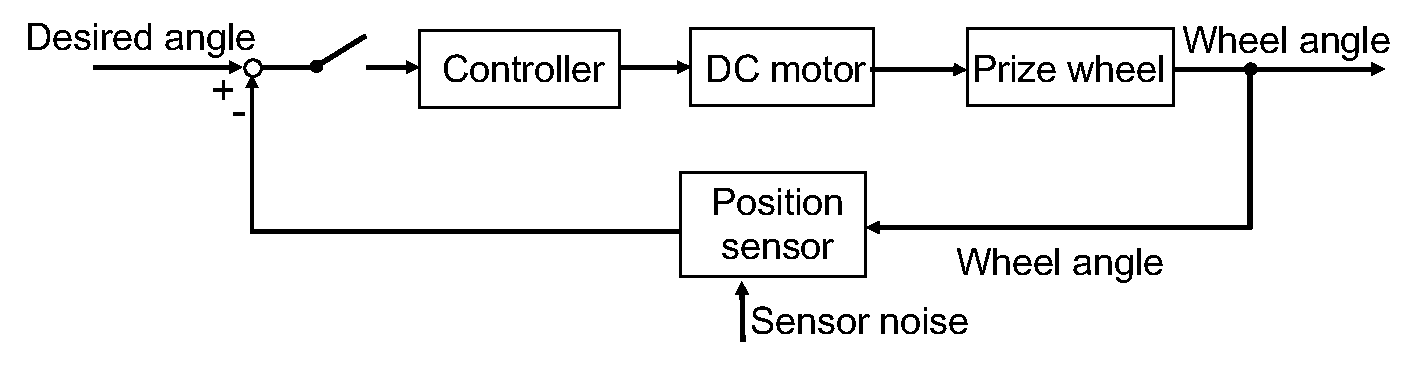
\includegraphics[width=.7\textwidth]{images/onoff.pdf}
    \begin{tikzpicture}[auto, node distance=1.5cm,>=latex',line width=1pt]
    \node [input, name=input] {};
    \node [sum, right of=input] (sum) {};
    \coordinate[right of = sum](switch){};
    \node [block, right= 1cm of switch] (controller1) {controller};
    \node [block, right= 1cm of controller1] (controller2) {DC motor};
    \node [block, right= 1cm of controller2] (controller3) {prize wheel};
    \coordinate [right=1cm of controller3, circle, scale=0.5, fill](tooutput){};
    \node [output, right=1cm of tooutput] (output) {};
    \coordinate [below= 0.2cm of tooutput] (measurements) {};
    \node[block, below= 1.5cm of controller2, pin={[pinstyle]below:noise}, node distance=3cm](controller4){position sensor};

    \draw [->] node[above=0.3cm]{desired angle}(input) -- (sum);
    \draw [-] (sum) to[normal open switch] (switch)-- (controller1);
    \draw [->] (controller1) -- (controller2);
    \draw [->] (controller2) -- (controller3);
    \draw [->] (controller3) -- node[above=0.3cm]{output angle} (output);
    \draw [-] (controller3) -- (tooutput) |- node[]{wheel angle}(controller4);
    \draw [->] (controller4) -| node[pos=1]{$-$} (sum);
\end{tikzpicture}

    \caption{On-off control system for a prize wheel}
\end{figure}
Take the example of the prize wheel. Position sensor measures the output angle, and compare this angle with the desired angle. Then use the switch\textit{(on-off)} to control the strength of the DC motor.

%-------------------------------------------%
\subsection{Gain (proportional) Control}
%-------------------------------------------%
\begin{itemize}
    \item Gain control applies control input that is proportional to the current error.
    \item It has very quick reaction to the current error
    \item But it is possible to \textbf{overshoot} when the error is magnified too much.
    \item Also, gain control leads to a non-zero \textbf{steady-state error}.
\end{itemize}

\begin{figure}[H] 
    \centering 
    % 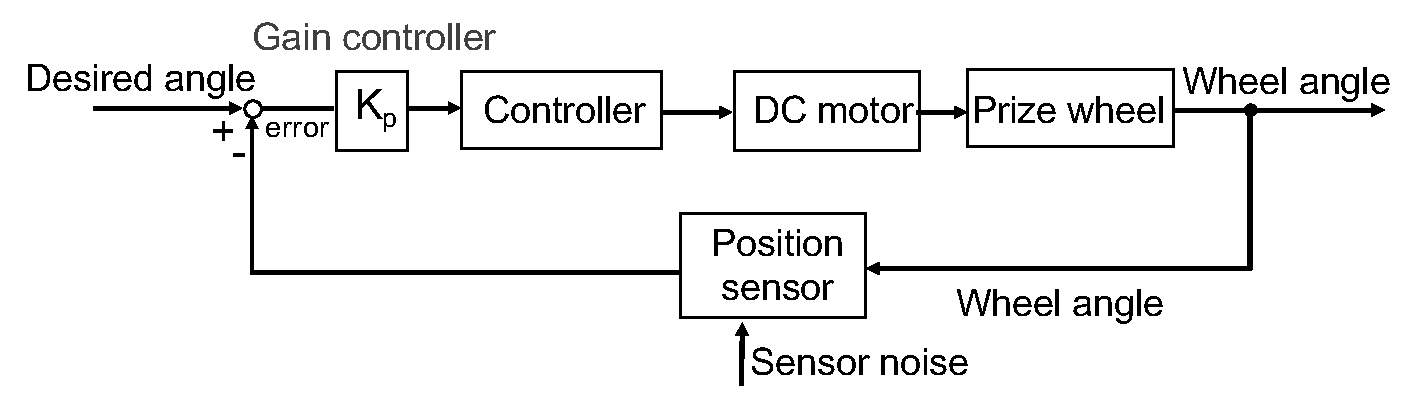
\includegraphics[width=.7\textwidth]{images/gain.pdf}
    \begin{tikzpicture}[auto, node distance=1.5cm,>=latex',line width=1pt]
    \node [input, name=input] {};
    \node [sum, right of=input] (sum) {};
    \node [block, right= 1cm of sum] (controller) {$K_{p}$};
    \node [block, right= 1cm of controller] (controller1) {controller};
    \node [block, right= 1cm of controller1] (controller2) {DC motor};
    \node [block, right= 1cm of controller2] (controller3) {prize wheel};
    \coordinate [right=1cm of controller3, circle, scale=0.5, fill](tooutput){};
    \node [output, right=1cm of tooutput] (output) {};
    \coordinate [below= 1.5cm of tooutput] (measurements) {};
    \node[block, below= 1cm of controller2, pin={[pinstyle]below:noise}, node distance=3cm](controller4){position sensor};

    \draw [->] node[above=0.3cm]{desired angle}(input) -- (sum);
    \draw [->] (sum) -- node[below]{error}(controller) node[above=.3cm]{{\color{gray} gain controller}};
    \draw [->] (controller) -- (controller1);
    \draw [->] (controller1) -- (controller2);
    \draw [->] (controller2) -- (controller3);
    \draw [->] (controller3) -- node[above=0.3cm]{output angle} (output);
    \draw [-] (controller3) -- (tooutput) |- node[]{wheel angle}(controller4);
    \draw [->] (controller4) -| node[pos=1]{$-$} (sum);
\end{tikzpicture}

    \caption{Gain control system for a prize wheel}
\end{figure}

Take the example of the prize wheel. The position sensor measures the wheel angle and compare it with the desired angle. The error is then calculated and sent into the gain controller. The gain controller magnifies the error and send to the DC motor for further action. 

%-------------------------------------------%
\subsection{PID Control}
%-------------------------------------------%
PID control is the most common controller used in industry which aims to reduce the tracking error between desired and measured output of the system.

\begin{figure}[H] 
    \centering 
    % 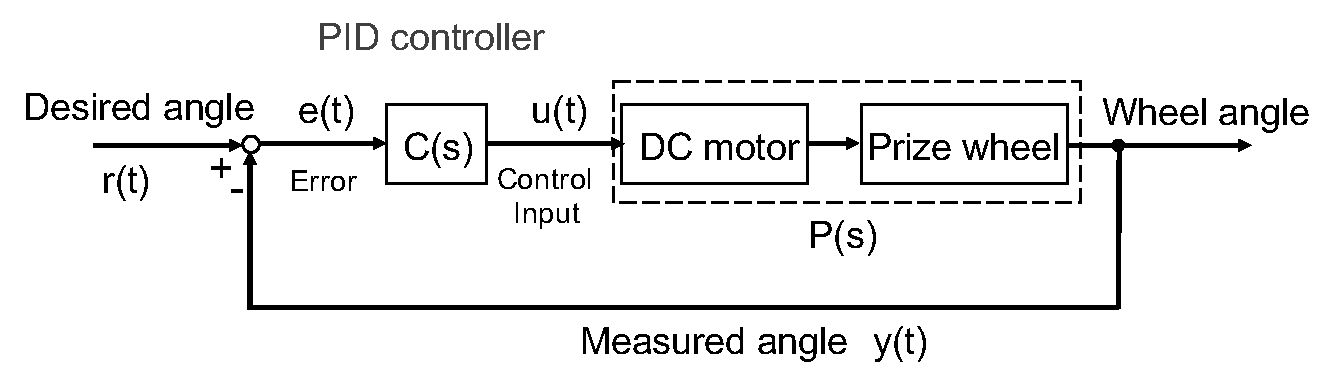
\includegraphics[width=.9\textwidth]{images/PID_control.pdf}
    % TikZ - PID controller

\begin{tikzpicture}[auto, node distance=1.5cm,>=latex',line width=1pt]
    \node [input, name=input] {};
    \node [sum, right of=input] (sum) {};
    \node [block, right= 1cm of sum] (controller1) {$C(s)$};
    \node [block, right= 1cm of controller1] (controller2) {DC motor};
    \node [block, right= 1cm of controller2] (controller3) {prize wheel};
    \coordinate [right=1cm of controller3, circle, scale=0.5, fill](tooutput){};
    \node [output, right=1cm of tooutput] (output) {};
    \coordinate [below= 1.5cm of tooutput] (measurements) {};

    \draw [->] node[above=0.4cm]{desired angle}(input) -- (sum);
    \draw [->] (sum) -- node[below=.2cm]{error} node[above]{$e(t)$}(controller1) node[above=.5cm]{{\color{gray} PID controller}};
    \draw [->] (controller1) -- node[below=.2cm]{control input} node[above]{$u(t)$}(controller2);
    \draw [->] (controller2) -- (controller3);
    \draw [->] (controller3) -- node[above=0.4cm]{output angle} (output);
    \draw [->] (controller3) -- (tooutput) |- (measurements) node[below=.2cm]{wheel angle, $y(t)$} -|  node[pos=1]{$-$} (sum);
\end{tikzpicture}
    \caption{PID control system for a prize wheel}
\end{figure}

\begin{itemize}
    \item Control input is the sum of \textbf{\underline{P}roportional}, \textbf{\underline{I}ntegral} and \textbf{\underline{D}erivative} of the error.
    
    \item Control input can be represented as:
    \[
    u(t) = K_{P}\  e(t)+K_{I}\int_{0}^{t}e(\tau)d\tau + K_{D}\frac{de(t)}{dt}
    \]
    
    \item PID controller can be represented as:
    \[C(s) =K_{P}+\frac{K_{I}}{s}+K_{D}s \]
    
        \begin{itemize}
             \item $K_{P}$ stands for \textbf{proportional gain}. It uses the information from the \textit{present error}.
             \item $K_{I}$ stands for \textbf{integral gain}. It uses the information from the \textit{past error}.
             It removes the steady-state error.
             \item $K_{P}$ stands for \textbf{derivative gain}. It uses the \textit{future error}. It improves the stability but has no effect on steady-state error.
        \end{itemize}
\end{itemize}

%-------------------------------------------%
\subsubsection{System response to $K_{P}$, $K_{I}$ and $K_{D}$}
%-------------------------------------------%
\begin{table}[H] \centering
    \begin{tabular}{|c|c|c|c|c|} \hline
        \textbf{Increase of} &\textbf{Overshoot}& \textbf{Rise Time} &\textbf{Settling Time}& \textbf{Steady-state error}\\ \hline
        $K_{P}$&Increase&  Decrease& Small increase& Decrease\\ \hline
        $K_{I}$&Increase &Decrease& Increase& Eliminate\\ \hline
        $K_{D}$&Decrease& Decrease& Decrease& No impact\\ \hline
    \end{tabular}
\end{table}

\begin{figure}[H] 
    \centering
    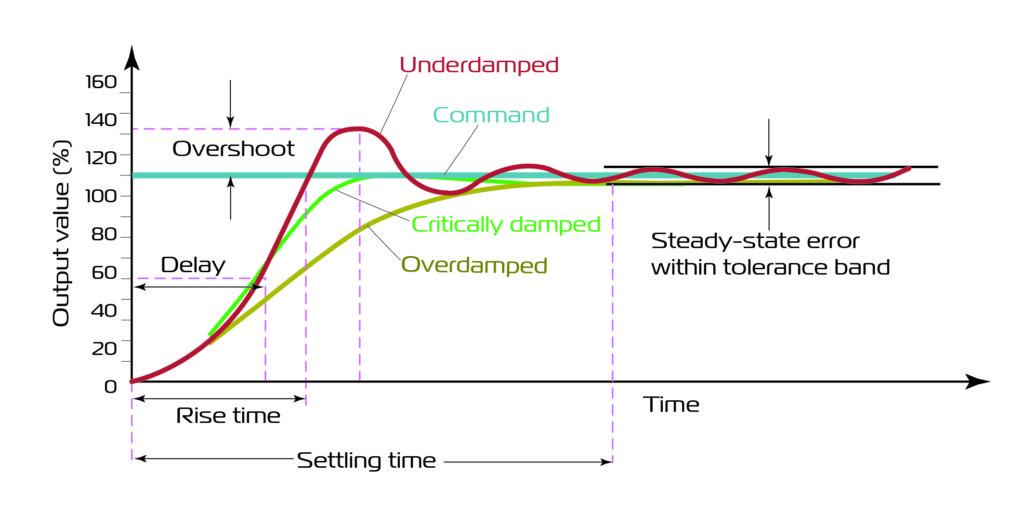
\includegraphics[width=0.8\textwidth]{images/PID_response.jpg}
\end{figure}